\documentclass{LULCSProject}
\usepackage{amsmath}
\usepackage{array}
\usepackage{enumitem}
\usepackage{listings, listings-rust, listings-js}
\usepackage{protobuf/lang} 
\usepackage{protobuf/style} 
\usepackage{graphicx}
\graphicspath{ {./figures/} }
\usepackage{todonotes}
\usepackage{hyperref}
\usepackage{url}

\newcommand{\tvect}[3] { \ensuremath{\Bigl(\negthinspace\begin{smallmatrix}#1\\#2\\#3\end{smallmatrix}\Bigr)}}
\newcommand{\twovect}[2] { \ensuremath{\left(\negthinspace\begin{smallmatrix}#1\\#2\end{smallmatrix}\right)}}

\title{An Open Source Smart home Platform}
\author{Niklas Harnish}
\date{12/05/2023}
%\BSc % \MEng \BEng etc. 
\supervisor{Dr Amna Asif}

\wordcount{0} % number of words in your report 


\abstract{Put your abstract here. You should create a short abstract (200
words at maximum) which is on a page by itself. The abstract should be
a very high-level overview: for example 1--2 sentences on the aims of
the project, 1--2 sentences on the kind of design, implementation, or
empirical work undertaken, and 2--3 sentences summarising the primary
contribution or findings from your work. The abstract appears in the
front matter of the report: after your title page but before the table
of contents.

what should go in here:
\list{}
    \item aims
    \item design
    \item implementation
    \item findings and primary contribution

}


\declaration{
  Put some text similar to the following in here:\\[.5em]
I certify that the material contained in this dissertation is my own work and does not contain
unreferenced or unacknowledged material. I also warrant that the above statement applies to the
implementation of the project and all associated documentation. Regarding the electronically
submitted work, I consent to this being stored electronically and copied for assessment purposes,
including the School's use of plagiarism detection systems in order to check the integrity of
assessed work.\\
I agree to my dissertation being placed in the public domain, with my name explicitly included
as the author of the work.\\
Name:\\
Date:
}

\dedication{
  If you want to dedicate to someone in particular
}

\acknowledgements{
  General acknowledgements \ldots

  your supervisor, your family, your
  friends, \ldots
}

\begin{document}

\maketitle

\pagenumbering{Roman}

\newpage
\listoffigures
\newpage
% \begingroup
% \let\clearpage\relax
\listoftables
%\endgroup

\newpage
\textbf{todo}:
\begin{itemize}
    \item add definitions for some terms: Crates vs Libraries, Traits vs Interfaces, Methods vs Functions and how they will be used within this paper
\end{itemize}

\pagebreak
\pagenumbering{arabic}

%%
%% include your chapters here
%%
\chapter{Introduction} \label{cha:intro}
\todo{actually write this section}Will write a couple of words about the project 
here, similar projects, inspirations etc. Citation here to remember how to do it 
:)

\section{Aims \& Objectives} \label{sec:intro:aims}
When researching available smart home technology, one major gap I came across 
was the availability of open source software. While options exist for someone 
interested in connecting their proprietary device to an open source platform 
(view \todo{find the link to this}), there was no solution for anyone looking to 
build their own device and then connect it to an open source hub. In fulfilling 
this goal, to build an open source platform for both devices and the hub they 
will connect to, there are multiple objectives that will need to be met along 
the way:
\begin{enumerate}
    \item Create a Library and API (Application Programming Interface) for 
        building smart home devices.
    \item Build a Server with an API for the smart home devices to communicate 
        with. This will act as a hub and will control clients connected to it.
         \begin{enumerate}
             \item This API should be well documented, so a user can interact 
                 with the hub, without using the Library.
         \end{enumerate}
     \item Create a frontend, which will be populated with devices currently 
         connected to the smart home. It will also be used to control clients 
         connected to the server.
         \begin{enumerate}
             \item The API provided by the server for this frontend should also 
                 be easy to use, so the user can create their own frontend 
                 environment.
         \end{enumerate}
     \item The code of all of the above should be hosted in a public repository, 
         with instructions for how to build and use every component of the 
         system.
         \begin{enumerate}
             \item An appropriate license should also be selected for this 
                 repository, so the code within it can be copied or modified by 
                 third parties.
             \item This repository should provide important links and provide 
                 information on the inner workings of the system, to support 
                 interested parties.
         \end{enumerate}
\end{enumerate}
    
\section{Project Overview} \label{sec:intro:overview} \todo{ask about this 
section}
\textit{Each bullet point below would give a small summary of the section}
\begin{enumerate}
    \item \textbf{Background Research} 
    \item \textbf{Design of the System \& Technology Decisions}
    \item \textbf{Implementation}
    \item \textbf{Results}
    \item \textbf{Conclusion and Reflection}
\end{enumerate}


% Always start your chapter on a new page!
\newpage
\chapter{Background} \label{cha:chapter2}

\section{IoT System Architectures} \label{sec:chap2:architectures}
Kamienski et al. describe a simple three layer architecture of an IoT system in \cite{DesigningOpenIotSystem}. Within this architecture, the top layer is the "Input System", from which any data that will influence the decisions of the IoT system will come from. Included in this are sensors, but also user facing interfaces. The second layer, known as the "Process System", is where any algorithms are run and system behavioral decisions are made. The goal of this layer is to gain an "improved understanding of the system where the  data comes from" \cite{DesigningOpenIotSystem}. The bottom layer is the "Output System", which are where decisions made by the Process System will be enacted. This is often represented as the devices connected to the IoT system.

This three layer architecture is expanded upon by Bansal and Kumar within \cite{IotEcosystemSurvey}, where three more architectures are described which expand upon the ideas within the three layer architecture. They are however more specialized than the three layer architecture. The first of these is a "Middleware Based" architecture, which can take many forms, but is usually combined with another type of architecture, with a middleware layer. The different types are described in detail by Zhang et al. in \cite{MiddlewareIOTSurvey}. The second is known as a "Fog Based" architecture, where certain tasks, usually those with less processing requirements, are calculated on device to reduce latency. More computationally expensive tasks are however calculated on a server in the cloud \cite{IoTArchitectures}.

The most relevant architecture to this report is known as a "Service Based" architecture (SBA). The SBA is defined around the concept of the Service Oriented Architectural (SOA) style \cite{InteractingSoaBasedIot} of software design. SOA is defined by the Open Group Foundation as an "architectural style that supports service-orientation", where a service is a "logical representation of a repeatable business activity that has a specified outcome" \cite{SoaSourceBook}. Each service is a "black box" any device interacting with it. Other devices use interfaces and API endpoints to make requests to the service and receive a result. A SOA is composed of many different services. In SBA, services are used to offer device functionality using interfaces, often using web based concepts such as SOAP or REST APIs \cite{TrustManagementSoaIot}. This allows devices with different capabilities and purposes to interact with the same system, allowing for an IoT system that is more flexible. 
\todo{Add section about which one I chose: Service Based Architecture}


\section{The Smart Home System} \label{sec:chap2:smarthome}
Sethi and Sarangi \cite{IoTArchitectures} define six components that need to be present within a social IoT setting. A social IoT system is defined as a IoT system where devices form relationships with other devices. While our smart home system will not be a social IoT system, some of these concepts are still of interest. These are: \todo{ask if this is ok with citation as its quite similar}
\begin{enumerate}
    \item ID: the device within the system needs to have a way of identifying 
        it.
    \item Meta-data: the device should have information regarding its form and 
        purpose
    \item Security Controls: the system should have some way of distinguishing 
        between different users. It should also be able to distinguish what 
        types of devices it can connect to or can connect to it.
    \item Service Discovery: each device should be able to discover other 
        devices connected to the system and what services they offer.
\end{enumerate}

There are some specific constraints specific to Smart Homes. Reliability is a key concern, due to the lack of a trained professional being available to fix any issues that arise. This is contrast to more industrial IoT settings, where there might be someone to fix any issues that arise. Another concern is the security and privacy of the system. Due to smart homes inherently having access to sensitive data (due to their position in someone's home), one must ensure that the system is both ethically sound and secure. The issue of security is further discussed in Subsection~\ref{sec:chap2:security}.
\todo{further add to this section, just not sure what yet}

\section{APIs and Web Interfaces} \label{sec:chap2:API}
The book "Designing Web APIs" makes an important distinction about APIs that can often be forgotten by developers. "Although APIs are designed to work with other programs, they’re mostly intended to be understood and used by humans writing those other programs" \cite{DesigningWebApis} (Chapter 1). Do to this reality, one must remember to design APIs appropriately. To help the API designer in doing that, there are multiple pre-defined architectural standards that they can use. 

\subsection{Request Response}
"Request Response" APIs (RRA) expose their interface through a web server, to which clients can make requests. A client will request data and will receive a response from the server. Common formats for requests and responses include JavaScript Object Notation (JSON) and Extensible Markup Language (XML). \cite{DesigningWebApis}. 

One popular type of RRA is known as Representational State Transfer (REST). Two important properties of REST is that it is used in Client-Server scenarios and that every request is stateless \cite{ArchitecturalStylesAPIs}. This means that every API request from the client to the server, must contain all information required to complete that request, without the server storing any of that information. Instead, all state is stored on the client. While this constraint might seem strange, it makes any API implementing REST easily scalable, and potentially easier/faster to build. The downside being inherently increased network traffic, with less control application behavior. \cite{ArchitecturalStylesAPIs}.

Another popular implementation of a RRA is known as the Remote Procedure Call Architecture (RPC). The key difference between RPC and REST is that RPC is about making an action on the server. In REST the client supplies the server with the information required to take an action, whereas using RPC the client tells the server what action to take. RPC APIs can usually express more nuance in their requests and are generally stateful. While RPC usually uses JSON or XML for requests and responses, there are multiple implementations, such as Google's gRPC and Apache Thrift, which do not. These are usually serialized and therefore consume less network traffic than non-serialized formats such as the aforementioned JSON \cite{DesigningWebApis}. 

\subsection{Event Driven}
Event driven APIs go in a different direction than RRAs. Instead of the client continuously requesting information from the server, the client registers with the Server once, then whenever there is an update the server sends the client a message notifying it of an update. This completely resolves the need for polling, the client continuously requesting updates from the server, which is often present in RAA API designs \cite{DesigningWebApis}.

Web sockets are a type of Event Driven API that utilize a bidirectional TPC connection between server and client. Unlike the previously mentioned API styles, a connection on a web socket stays active until closed \cite{WebsocketStandard}. Due to the bidirectional TCP connections both client and server can send one another packets, even at the same time \cite{DesigningWebApis}. This is in contrast to REST and RPC protocols, where only the client can contact the server. This comes at the downside of scalability, as a server must maintain a connection with every device that is connected with the server. Additionally, there are also issues when a client is on an unstable connection, as web sockets expect a client to stay connected, with the client having to reinitiate the connection if it is dropped \cite{DesigningWebApis}.

The final type of API that deserves a short mention is the Web Hook. Web hooks work in an unconventional manner, where the initiator of an exchange gives a URL to their own API endpoint. This URL is then used by the receiver. Whenever a new event for the initiator occurs, the receiver will send information about the event to the URL \cite{DesigningWebApis}. While at face value this may seem like an obvious solution in an IOT based environment, where devices are often waiting for an event from the central server, it makes less sense when one realizes that every device connected to this webhook will need to host some sort of HTTP server, to receive the API requests. This makes it unsuitable, especially in environments where IOT devices are low powered, embedded systems devices. Web hooks are often used in server to server communication, as in such a scenario they are trivial to set up (as servers will most likely already be setup to receive API requests) \cite{DesigningWebApis}.
\todo{Add section about which one I chose: RPC, specifically gRPC}

\section{Security} \label{sec:chap2:security}
Requires more research and testing to find a good solution, will be written and implemented later.\todo{Remove this text and write this section}

\section{Networking} \label{sec:chap2:networking}
I don't think this section is very interesting, so I will probably not write about this in background, however it will be mentioned in the implementation, that I left it mostly up to the user\todo{Remove this text}

\section{Open Source and Licensing} \label{sec:chap2:opensource}
Not sure about this section either, perhaps speak about how some open source projects are managed and different possible licenses. This does not sound interesting either.\todo{Remove this text}

\todo{write another section about the general planned architecture of the system, including system layers, components, how they are connected to each other}


\newpage
\chapter{Design} \label{cha:design}
\section{Technology Choices} \label{sec:chapdesign:technology}
This section will discuss choices that have been made throughout the project regarding technology used and justifications for their usage.

\subsection{Rust} \label{sec:chapdesign:technology:rust}
There were a few requirements when choosing an appropriate programming language for this project:
\begin{enumerate} 
    \item Performance: There are two aspects to performance within this project. Performance considerations and optimization are vital on IOT devices themselves, due to their limited on-board processing power. On the other hand, while performance on servers is definitely important, it is significantly easier to scale server-performance, by simply adding more servers (horizontal scaling) or by improving the hardware of any individual server (vertical scaling), than it is to improve performance of an IoT device. This is especially true of an IoT device that is already deployed.
    \item Stability: Another important requirement when choosing a language is the stability of code written in the language. This does not necessarily mean that code written in any language is inherently unstable. This requirement is more of a consideration about if a language enables and encourages a programmer to write code that is memory-safe and handles errors correctly. This is important in an IoT environment, as devices are expected to run for long periods. What is the point of a security camera if it's software crashes every couple days, due to an obscure memory out of bounds error? 
    \item Security: While no language is inherently "hack-proof" or secure, there are ways a language can encourage behaviors that can lead to better outcomes in security. A blog-post by the "Microsoft Security Response Centre" states that 70\% of all vulnerabilities assigned a CVE (Common Vulnerabilities and Exposures) each year are due to memory corruption errors \cite{ProactiveApproachToSecureCode}. In the post the languages "C" and "C++" are specifically referred to as being part of this problem. As mentioned in subsection ~\ref{sec:chap2:security}, security is of particular importance in smart home systems, so ensuring a method or language that enables secure code is chosen is of particular importance. 
    \item Ease of Use and Comfort: While not particularly important in the final product, having a language that is easy to develop in can make the developer experience easier and can lead to faster iteration on ideas, perhaps leading to a better final result. That being said, developer familiarity with a language can more than make up this difference. A seasoned C++ developer will be able to iterate faster and produce a better product in C++, than if they are using an "easy" language, that they are not as familiar with.
\end{enumerate}\todo{not sure I like the list style here}
After some deliberation, the language that was chosen for this project was Rust. While C/C++'s performance rivals and often surpasses Rust, the difference is often quite marginal \cite{PerformanceEvalOnMicrocontroller}, due to all three being compiled to machine code. What makes Rust different, is its headline feature, known as the "borrow checker". While the details of the borrow checker are out of scope of this paper, it can ensure that at compile-time, the code is memory safe. While there are ways to circumvent this (using the "unsafe" keyword), this has to be explicitly done. Due to the code being guaranteed memory safe at compile time, outside the aforementioned unsafe blocks, Rust code is known for its ability to run long-term without running into crashes. Additionally, Rust code is a popular choice for embedded devices, due to being able to compile without a standard library (this has to be enabled), giving it flexibility in a project such as this.

I have decided to use Rust for both the Server and Clients. While Rust might be a somewhat obvious choice for IoT clients, it is less so for servers. Due to the "borrow checker", while Rust might be safe, it is often said to be harder to write than traditional languages. This makes it more questionable as the primary language for the server, due to it being a less constrained platform (view performance section above). While servers are theoretically almost infinitely horizontally scalable, in practice this is often not the case, especially in a smart-home's case, as they have to fit in someone's home and generally should be affordable. Therefore, ensuring that the server can run on as many devices as possible, be it a Raspberry-Pi, or a modern desktop, is an important goal to strive for. The "difficulty" aspect of Rust can be largely counteracted by personal familiarity with the language. Additionally, having a stable server is very important, especially since all IoT devices will need to frequently communicate with this server, an aspect which Rust excels at. Rust also has a thriving community of libraries (known as crates), which using the language gives access to. For these reasons I have chosen Rust as the primary programming language of the Server and Client parts of this project.

Note that the words crate and library will be used interchangeably throughout this report, due to them being very similar concepts, but library being more familiar to non-rust users. 

\subsection{gRPC} \label{sec:chapdesign:technology:grpc}
gRPC is an RPC implementation released by Google in 2015. It uses Protocol Buffers (protobufs) as an interface definition language (IDL), to define services on servers, that clients can then call, such as any RPC library. The server runs a gRPC server and the client runs the gRPC client \cite{grpcHomepage}. Protobufs are compiled to many different languages, with many different libraries available for these languages, that automate much of the process. In a performance comparison between REST, gRPC, websockets, GraphQL, gRPC came out ahead in many different metrics \cite{reviewOfInternetProtocols}. These include: 
\begin{itemize}
    \item inserting one value into a database
    \item fetching one value from a database 
    \item fetching one hundred elements  
\end{itemize}
in both native and containerized tests. In fact, gRPC was the most performant internet communication protocol in all metrics apart from memory usage.

Due to its performance and cross-language support I have chosen gRPC as the internet communication protocol for this project. The specific library used for this project is known as "Tonic". Tonic is a Rust gRPC crate that includes both a gRPC server and client. It also utilizes "prost" to compile protobuf files into Rust code, without having to interface the protobuf compiler itself. All protobuf files are compiled as a compilation step of the server and client, eliminating the need for external build scripts (this is only partially true, view Sub Section~\ref{sec:chapdesign:server:protoBufs}).

\subsection{Typescript \& VueJS} \label{sec:chapdesign:technology:ts}
While a Command Line Interface (CLI) frontend, written in Rust, will be made available, the main focus will be on the Graphical User Interface (GUI). To ensure that it can run on a variety of systems and is relatively easy to create, it will be web based, using Javascript at runtime. However, it will be written in Typescript. Typescript is a superset of Javascript, that compiles to Javascript and leaves no trace of types behind. Typescript provides a robust type-system, including, but not limited to \cite{understandingTypescript}:
\begin{itemize}
    \item Structural type equivalence, instead of Javascript's by-name type equivalence
    \item Types and concepts for object-based programming
    \item Type operators
\end{itemize}
All of these, while not guaranteeing that the program will be type-safe at runtime, help a developer design more robust and long term solutions generally associated with statically typed languages.

In conjunction with Typescript a web-development framework will be used. Web frameworks are libraries for Javascript that allow easier development of websites and web apps, often incorporating HTML (HyperText Markup Language) and CSS (Cascading Style Sheets) code into Javascript code. They also provide reactivity, meaning that if a variable changes in the code, that change can easily be reflected on the site. This can be done in most frameworks by simply using the variable in the HTML code, something that standard HTML does not support (methods of doing this differs between frameworks).

Most of the choice between different web-frameworks comes down to personal preference and familiarity with a framework. That being said there can be performance differences between different frameworks, that could make a difference on some systems. While there is a lack of formal experiments on framework performance, an informal experiment \cite{performanceComparisonJS} showed that while there is a performance difference between different frameworks, it should not be the primary decision maker. When the difference when creating 1000 rows between vanilla JavaScript and VueJS is 32 milliseconds, the disparity will not be noticeable to the end user. For this reason, and personal familiarity with the framework, I have decided to use VueJS as the frontend development framework for this project.

\subsection{Raspberry Pi} \label{sec:chapdesign:technology:raspi}
\todo{write this}

\section{System Architecture} \label{sec:chapdesign:architecture}

\section{Security} \label{sec:chapdesign:security}
As previously discussed, security is an important concern within a smart-home environment. The user of the system is putting trust into the system to behave as it is meant to, while keeping their personal data safe from outside intruders. That is why special care will be put into the security aspects of the system. This will come in a two pronged approach using certificates and signatures. 
\subsection{Certificates}
A certificate is a tool for verifying that a client is who they say they are. It is generated by the server and can be verified by the server. This is useful, for example, if the client goes offline and at a later time wants to re-aunthenticate with the server. They can send the certificate provided to them earlier and the server can verify it. The certificate scheme that will be implemented is based on \cite{disSysConceptsDesign}.

Figure~\ref{fig:certificate_exchange} shows the certificate exchange protocol that will be used, where cK is the client key pair and sK is the server key pair. K(pub) represents the public key part of the key pair.
\begin{figure}[h]
\caption{Certificate Exchange}
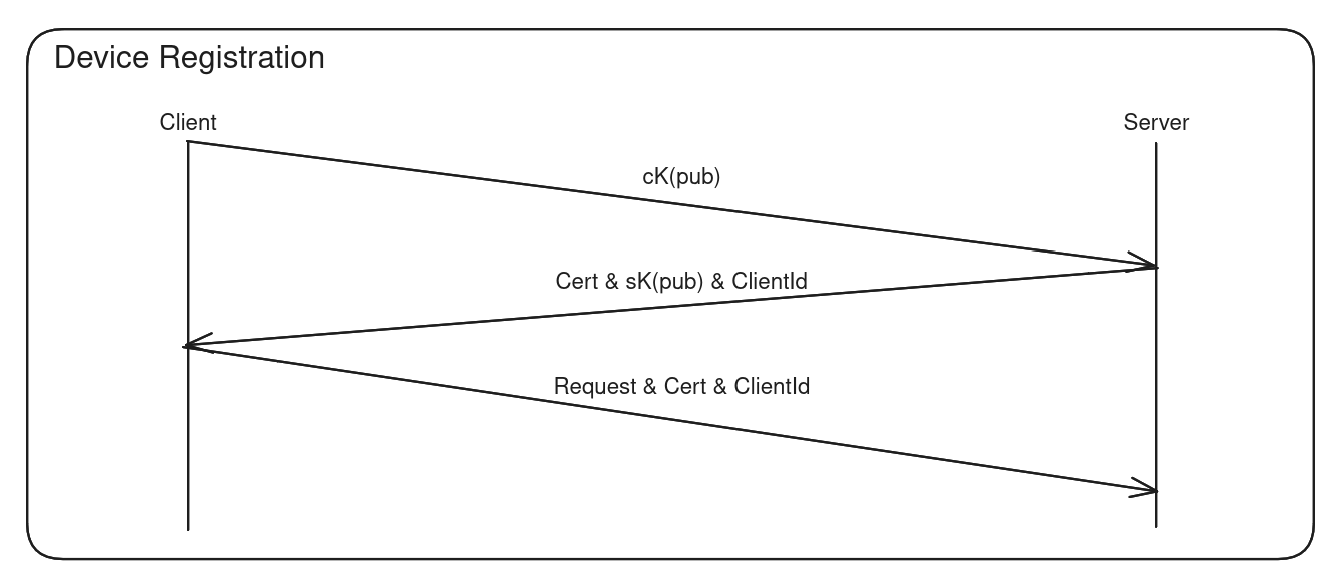
\includegraphics[width=\textwidth]{certificate_exchange.png}
\label{fig:certificate_exchange}
\end{figure}

At startup the server and client will both generate an asymmetric key pair using the Rivest, Shamir, Adleman (RSA) public key system. Then, during registration, the client will send the server their public key. The server then creates csr where \(csr = cK(pub) + ClientId\). Csr is then hashed using SHA256 hashing to create the certificate: \(certificate = H_x(csr)\). This certificate is then sent back to the client, along with the server public key and their client identifier (which is a UUID randomly generated by the server). Now, if the client goes offline and wants to re-register, instead of having to repeat the registration process again, they can simply include their certificate instead and be verified by the server. Verification is quite simple. The client simply re-generates csr using the client's public key and client-id, then re-hashes them. If the new hash is the same as the certificate, then the client is verified.

\subsection{Signatures}


\newpage
\chapter{Implementation} \label{cha:implementation}
This chapter aims to provide a low-level, in-depth explanation of how a variety of systems work throughout the project's codebase. It provides code samples, with explanations of what that code is doing, to give insight into how this project was built. It does this through describing all aspects of the Registration Service. Throughout, how devices connect using the Registration Service, how these devices are registered in the server and how this information is reflected on the frontend are described in detail. This information can then be extrapolated to the other services present within the overall system.

\section{Backend Server \& Device Management} \label{sec:chapimpl:server}
Due to the server being the largest part of this project, and practically being a requirement for testing the client and frontend functionality, this will be focused on first. This section will describe defining and compiling protobuf files for API endpoints, server startup, how IOT devices are registered, security mechanisms and how concurrency was handled within the server. 

\subsection{Protocol Buffers} \label{sec:chapimpl:server:protoBufs}
\todo{I think this section should be shortened}

Remote functions accessible through gRPC are defined in ".proto" files. They use a fairly basic syntax, where the user can define a service using the "service" keyword. A service can contain many functions which a client can call, these are defined using the "rpc" keyword. Structs are defined using the "message" keyword, where each field is separated by a semicolon. These structs will then be compiled to their corresponding datatype in whatever language you are using. For example, they are compiled to classes in Typescript or structs in Rust. This makes them useful if a datatype is shared between languages,  they can be defined in one protbuf file and used across languages. Protobuf structs contain fields, which can have multiple modifiers, including optional and repeated. Repeated marks a field as possibly being a list, or array structure, optional marks a field as optional (represented differently between languages). Finally, messages from other files can be imported. Below is the service definition for the RegistrationService, found in \textbf{\textit{protos/iot/registrationService.proto}}:

\begin{lstlisting}[language=protobuf3, style=boxed]{iot/registrationService.proto}
syntax = "proto3";
package iot.registration;
import "types.proto";

service RegistrationService {
    rpc Register(
        RegistrationRequest
    ) returns (RegistrationResponse);
};

message RegistrationRequest {
    string public_key = 1;
    string name = 2;
    repeated iot.types.DeviceCapabilityStatus 
        capabilities = 3;
}

message RegistrationResponse {
    string public_key = 1;
    string client_id = 2;
    string certificate = 3;
}
\end{lstlisting}

Here we define a service called "RegistrationService", with a function called Register. This function is called by IOT clients when they first attempt to connect to the server which takes a RegistrationRequest as a parameter and returns a RegistrationResponse. The file also defines two "messages". The capabilities field is repeated, meaning it is an array data structure. This array contains the type DeviceCapabilityStatus, which is defined in iot.types. We can see this type is imported at the top of the file, from "types.proto". This is the definition of DeviceCapabilityStatus:

\begin{lstlisting}[language=protobuf3, style=boxed]{iot/types.proto}
message DeviceCapabilityStatus {
    bool available = 1;
    string capability = 2;
}
\end{lstlisting}

In summary, if an IOT device wants to register with this server, they will need to call the Register server stub. The server stub takes one parameter, the RegistrationRequest message. This message requires the client to give it's public key, it's display name and an array of "DeviceCapabilityStatus". The Register function then returns a RegistrationResponse. To see how this service is implemented on the server, view subsection~\ref{sec:chapimpl:server:registration}.

\subsection{Server Start Up} \label{sec:chapimpl:server:startup}
This section will describe what is done when the server first starts. It will give a general overview of startup and the details of starting a gRPC and HTTP server in Rust. For more details, view the main function within \textit{\textbf{/backend/src/server/server.rs}}.

Startup of the server is currently quite simple:

\begin{figure}[h]
\caption{Simplified Diagram of Server Startup}
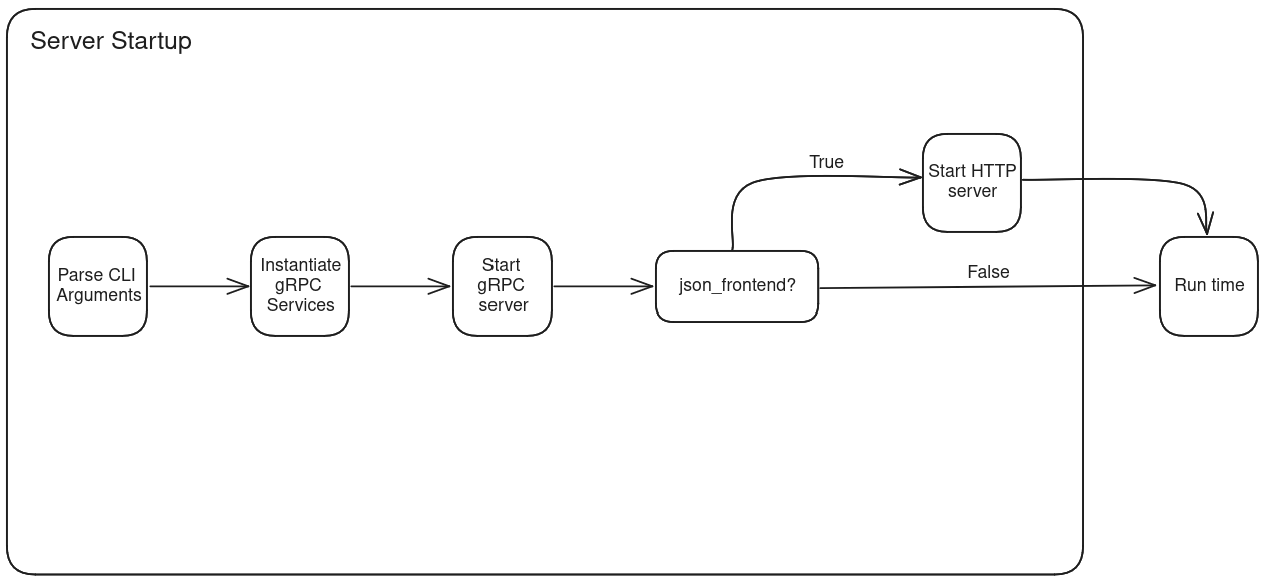
\includegraphics[width=\textwidth]{server_startup}
\end{figure}

\subsubsection{Command Line Arguments}
Command line (CLI) arguments are parsed using a Rust library called "Clap". Currently the only commandline argument that can be passed is running the optional HTTP server, which enables using JSON for the frontend (view subsection~\ref{sec:chapimpl:frontend:json}), however there are plans to include other arguments, such as giving an IP address or Port for the gRPC server to run on as an argument. Currently, the computer's IP address is discovered automatically using a crate called "local-ip-address". 

\subsubsection{Creating gRPC Services}
Next gRPC services are instantiated. GRPC services in Rust take the form of structs that implement the trait (interface) defined as a service within a protbuf file. Take for example, the "RegistrationService" from \textbf{\textit{protos/iot/registrationService.proto}}, defined in subsection~\ref{sec:chapimpl:server:protoBufs}:
\begin{lstlisting}[language=protobuf3, style=boxed, showstringspaces=false]{}
service RegistrationService {
    rpc Register(
        RegistrationRequest
    ) returns (RegistrationResponse);
};
\end{lstlisting}

This is implemented on a struct in Rust like this (code snippet from \textit{\textbf{backend/src/server/registration.rs}}):
\begin{lstlisting}[language=Rust, style=boxed, showstringspaces=false]{}
use self::registration_service
    ::registration_service_server::RegistrationService;

#[async_trait]
impl RegistrationService for ClientRegistrationHandler {
    async fn register(
        &self,
        request: tonic::Request<
            self::registration_service::RegistrationRequest
        >,
    ) -> RPCFunctionResult<
        self::registration_service::RegistrationResponse
    > {
        //code goes here
    }
}
\end{lstlisting}

Where "RegistrationService" is an interface, defined in a protobuf file (view subsection~\ref{sec:chapimpl:server:protoBufs}). "ClientRegistrationHandler" is the name of the struct this interface is being implemented on. If the interface is implemented correctly, this struct is now a service and, after being handed to the gRPC server struct, this function can then be called using a RPC through gRPC. In other words, any gRPC client that is connected to this gRPC server can now call this function, as long as their programming language supports it.

\subsubsection{Starting the gRPC Server}
After implementing all services defined in the protobuf files on appropriate structs, the gRPC server can now be started. This is done in the following code snippet from \textit{\textbf{/backend/src/server/server.rs}}:
\begin{lstlisting}[language=Rust, style=boxed, showstringspaces=false]{}
use registration_service_server::RegistrationServiceServer;

let registration_service =
    registration::ClientRegistrationHandler::new();
let grpc_server = tonic::transport::Server::builder()
    .add_service(
        RegistrationServiceServer::new(
            registration_service,
        )
    )
    .serve_with_shutdown(
        grpc_address,
        tokio::signal::ctrl_c().map(drop)
    )
    .await;

println!("Started GRPC Server on {}", grpc_address);
\end{lstlisting}
\textit{Note that the above code snippet is abbreviated for readability, it is however still valid Rust code and gives a good representation of what is done in server.rs.} 

The Server struct we are instantiating on line 1 comes from the transport module within the tonic crate. We invoke the builder method on the Server struct, a very common pattern within the Rust ecosystem. In fact, the same pattern is used instantiate a new IoT device in the client library for this project (view section~\ref{sec:chapimpl:devicelib}). After invoking the builder method, which returns a new Server struct, we add structs that implement the aforementioned services to it, using the "add\_service" method. In our case, we want to hand it a "RegistrationServiceServer" struct, provided by the protobuf file. The "new" method on the "RegistrationServiceServer" takes one argument, which is a struct that implements the "RegistrationService" trait, which is the trait we implemented on our ClientRegistrationHandler earlier. We therefore hand it the variable "registration\_service" which is of the type "ClientRegistrationHandler".

The "server\_with\_shutdown" method consumes the Server struct and runs the server, on the address handed to it in the parameter. In this case it is the variable "grpc\_address", which is a string which contains the device's IP address and a port. The second parameter simply tells Rust to drop the gRPC server (shutdown and gracefully free the memory associated with it) when the key combination crtl-c is pressed. This is an easy way to implement this behavior in Rust when working with multiple threads (view subsection~\ref{sec:chapimpl:server:threads}).

Once we have added all services to the Server struct, it must be awaited using the "await" keyword. For more information on how this works view subsection~\ref{sec:chapimpl:server:threads}.  

\subsubsection{Starting the HTTP Server}
Starting the HTTP server works almost the same as the gRPC server, using the same builder pattern. However, this time instead of using the Tonic crate, we are using a crate named "Actix", a self-described "powerful, pragmatic, and extremely fast web framework for Rust" \cite{actixWebsite}. View part of the "run\_json\_frontend" function, found in the file \textbf{\textit{backend/src/server/server.rs}} below:
\begin{lstlisting}[language=Rust, style=boxed, showstringspaces=false]{}
const JSON_ADDRESS: &str = "localhost:50052";

let result = actix_web::HttpServer::new(move || {
    actix_web::app::App::new()
        .app_data(web::Data::new(json_state.clone()))
        .service(json_registration::json_registration)
})
.bind(JSON_ADDRESS)?
.run()
.await;
\end{lstlisting}
\textit{Note that the above code snippet is abbreviated for readability, it is however still valid Rust code and gives a good representation of what is done in server.rs.} 

Due to this builder function requiring more Rust specific knowledge to understand, it will be simplified here. It is functionally the same as the one seen from Tonic. First we create a new HTTPServer struct from the actix\_web module. We then hand it our services using the "service" method. What is different here, is that we are actually handing it callback functions, instead of structs with traits implemented. To view an example of these services, view subsection~\ref{sec:chapimpl:server:registration}. From there we bind this server to the constant string JSON\_ADDRESS. This is an IP Address defined at compile time, the definition however is found above the web server. The server is running on localhost, as it is meant for communication with the web frontend. We then call the run method and await the result. In reality the server is being awaited on a different thread than the gRPC server, so the two can run concurrently. This is not shown in the above code snippet. 

For code beyond the above provided abbreviated snippets view the file \textbf{\textit{backend/src/server/server.rs}}, which contains the main function for the server.

\subsection{Device Registration} \label{sec:chapimpl:server:registration} 
This section will give an overview of the server's response to a device registration attempt. For information about how registration is performed on a device, view subsection~\ref{sec:chapimpl:devicelib:registration}

Figure~\ref{fig:server_registration} shows the process of the server receiving a registration request from a client:
\begin{figure}[h]
\caption{Simplified Diagram of Device Registration}
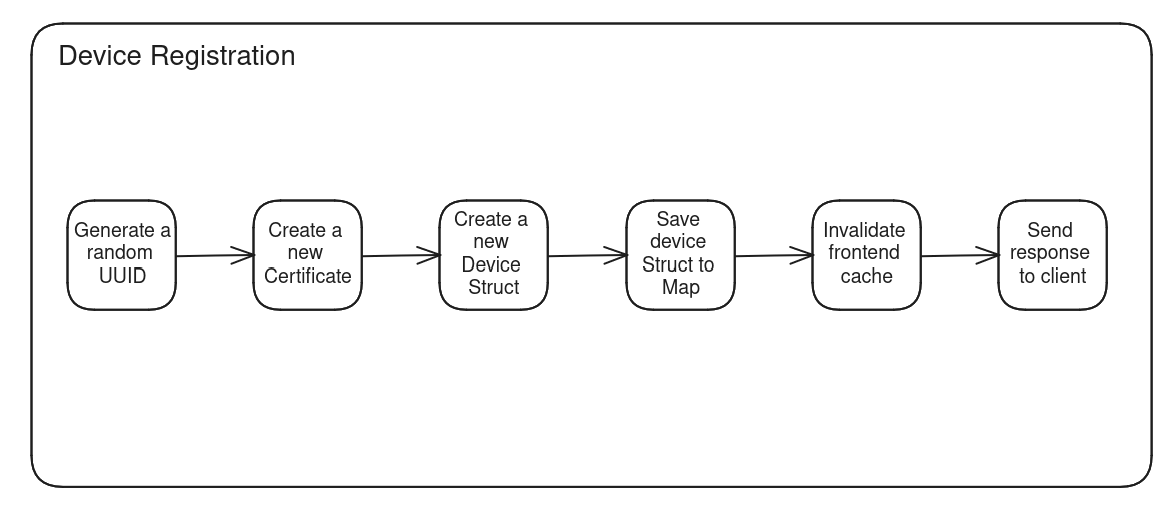
\includegraphics[width=\textwidth]{device_registration}
\label{fig:server_registration}
\end{figure}

When a device wants to connect to the server, it uses the "Register" function from the "RegistrationService" through gRPC. To do so, it must first create a "RegistrationRequest", the contents of which are detailed within the \textit{\textbf{proto/iot/registration.proto}} protobuf file:

\begin{lstlisting}[language=protobuf3, style=boxed, showstringspaces=false]{}
message RegistrationRequest {
    string public_key = 1;
    string name = 2;
    repeated iot.types.DeviceCapabilityStatus 
        capabilities = 3;
}

//from proto/iot/types.proto
message DeviceCapabilityStatus {
    bool available = 1;
    string capability = 2;
}
\end{lstlisting}
This is the same protobuf code detailed in subsection~\ref{sec:chapimpl:server:protoBufs}. The "RegistrationRequest" contains the device's public key and its display name. The public key will be used for encryption and signing, the name is what the device is called on the frontend-interface. The final field is an array of type "DeviceCapabilityStatus", which is a message (struct) with two fields. A capability in this system represents something the device can do. This takes the form of a string. If a capability is available, that means the server relays that capability to any frontend devices connected to the server. If it is not available, the server still keeps that information, but does not relay it to frontends. 

A simple example of a capability is one for a lamp. A lamp could have two capabilities, "turn on" and "turn off". If the lamp is off, the capability "turn on" is available to the user. If the user decides to invoke that capability, the lamp will turn on, the "turn on" capability will no longer be available and the "turn off" capability will become available. 

This system has much room for extension, with some glaring features that need to be added being:
\begin{itemize}
    \item Optional variables attached, such as a float value. Could be used for turning up a speaker for example.
\todo{still planning to implement this before deadline, add more stuff here}
    \item Access levels, only an admin can see this capability.
\end{itemize}

The device sends this registration request to the server. With the information from the request, the server can then register the device in a HashMap, which maps the device UUID to the Device struct, following the steps described in figure~\ref{fig:server_registration}. The Device struct is defined in \textit{\textbf{/backend/src/server/device.rs}} as:
\todo{fix this code snippet}
\begin{lstlisting}[language=Rust, style=boxed, showstringspaces=false]{}
use crate::types::types::DeviceCapabilityStatus;
#[derive(Clone)]
pub struct Device {
    pub name: String,
    pub uuid: Uuid,
    pub stringified_uuid: String,
    pub active_capabilities: Vec<DeviceCapabilityStatus>,
    pub inactive_capabilities: Vec<DeviceCapabilityStatus>,
    pub device_public_key: rsa::RsaPublicKey,
}
\end{lstlisting}
The structure of a device is quite self-explanatory, the only thing of note is having the UUID as two fields, one time as the UUID struct and once as a string. This is due to the type conversion being done very often in certain sections of code, it made sense to do this conversion once and reuse it.  

\subsection{Device \& Server Communication}
Device and Server communication happens through polling. Every 0.5 seconds the device sends a request through the "RequestUpdateService" to the server. The service is defined in the \textit{\textbf{/protos/iot/requestUpdateService.proto}} file:
\begin{lstlisting}[language=protobuf3, style=boxed, showstringspaces=false]{}
service RequestUpdateService {
    rpc PollForUpdate(PollRequest) returns (PollResponse);
};
\end{lstlisting}
The "RequestUpdateService" has one function, named "PollForUpdate". It accepts a "PollRequest" as a parameter and returns a "PollResponse". When a device requests an update from the server, it must provide its UUID, certificate, a timestamp of when it was sent and the signature of the message, so the server knows what device is requesting and so the server can ensure that the device is who it says it is. Additionally, it provides it's updated list of capabilities. Below is some pseudocode to show how the server creates a response (you can view the real function in file \textit{\textbf{backend/src/server/polling.rs}}): \todo{add signature to this}

\begin{lstlisting}[language=Python, style=boxed, showstringspaces=false]{}
def poll_for_update(self, request):
    device = self.connected_devices.get(request.uuid)
    if device == null:
        return PollResponse(
            has_update: PollingOption::DeviceNotFound,
            updates: [],
        )

    if !request.updatedCapabilities.is_empty():
        active_capabilities, inactive_capabilities = (
            request.updatedCapabilities.partition(
                (capability) => capability.available == True
            )
        )
        device.replace_capabilities(
            active_capabilities,
            inactive_capabilities
        )

        self.frontend_cache_valid = false

    updates = self.updates.get(request.uuid)
    if updates.is_empty():
        return PollResponse(
            has_update: NONE,
            updates: [],
        )

    updates_clone = updates.clone()
    updates.clear()

    return PollResponse(
        has_update: SOME,
        updates: updates_clone
    )
\end{lstlisting}
When the poll\_for\_update function receives a request, it first checks if the device has updated capabilities. This can happen if something has changed with the device since the last poll or since registration. If the device has updates capabilities, then they are replaced and the frontend cache is invalidated. The frontend cache being invalidated means that some values need to be recalculated next time a frontend requests information about this device, instead of simply using the previous values.

Next the function checks if any events are available for the device in question. Events are created by the user on the frontend. For example, when the frontend activates capability "turn\_on", an event is created on the server for the corresponding device. When the device then requests updates, this event is sent to the device and the device can respond accordingly. The server will include in the poll response, an indicator if new events are available, or an error code. If events are available they will also be included in the message.

When the client receives the response to their poll, they can then decide what to do with the events they have received, the server does not define any behavior. It simply reports to the client any events that have happened. This choice was made to enable a programmer to better define device behavior themselves and prevents issues with the server and device being out of sync about what behaviors are available. The downside of this, is that the server cannot guarantee to the frontend that anything has happened when a button is clicked. It also cannot give feedback until the event is processed by the IoT device. Another downside is that it leads to more calculation being done on the IoT device itself and can potentially lead to lost updates if the device itself malfunctions.


\subsection{Threads \& Concurrency} \label{sec:chapimpl:server:threads}
\todo{write this}

\section{Device Library \& Example Device} \label{sec:chapimpl:devicelib}
Another goal of this project was to create a library that can be used by other programmers, to easily create an IoT device that can connect to this system. This library was written for use with Rust. It is published within the Rust library ecosystem website, found at \textit{crates.io}. The library entry on \textit{crates.io} can be found be \textbf{\href{https://crates.io/crates/NOSHP-Client}{here}}. 

\subsection{Using the Library}
\todo{some of this code has outdated code fix that}
The main purpose of the library to is to abstract details of how the client \& server connection works away from the programmer. While they can still view the source code due to it being open source, they should not need to know the inner workings of the library to be able to use it. The example below, which can be found within the repository for the example device \textbf{\href{https://github.com/niknik3610/Example-Iot-Device}{here}}, demonstrates usage of the library to create a simple IoT device. The purpose of this device is to toggle an LED, attached to a general purpose input output (GPIO) pin, on and off when the appropriate event is received. This code is made to run on a Raspberry Pi and will therefore not run on non Raspberry Pi Devices. It uses a combination of the NOSHP\_Client library (the library created within this paper) and rrpal, a library commonly used to interact with the Raspberry Pi's GPIO in Rust. View the entire code for this simple IoT device and an in-depth explanation of it below: 

\begin{lstlisting}[language=Rust, style=boxed, showstringspaces=false]{}
use NOSHP_Client::{
    client::{ClientHandler, Request, State},
    client_config::{ClientConfig, ParsedConfig},
};
use std::error::Error;
use rppal::gpio::{Gpio, OutputPin};

struct ExampleState {
    led_pin: OutputPin,
}
impl State for ExampleState {}
impl Default for ExampleState {
    fn default() -> ExampleState {
        return ExampleState {
            led_pin: Gpio::new()
                .unwrap()
                .get(GPIO_LED_PIN)
                .unwrap()
                .into_output(),
        };
    }
}

const GPIO_LED_PIN: u8 = 2;
const CONFIG_PATH: &str = "./example_config.toml";
#[tokio::main]
async fn main() -> Result<(), Box<dyn Error>> {
    let config = 
        ClientConfig::load_config(CONFIG_PATH).unwrap();

    let client_handler = ClientHandler::new()
        .add_callback("Turn On", Box::new(turn_on_led))
        .add_callback("Turn Off", Box::new(turn_off_led))
        .run(config)
        .await
        .unwrap();

    return Ok(());
}

fn turn_on_led(state: &mut ExampleState, req: Request) {
    state.led_pin.set_high();
    println!("set pin {} to high", GPIO_LED_PIN);
}
fn turn_off_led(state: &mut ExampleState, req: Request) {
    state.led_pin.set_low();
    println!("set pin {} to low", GPIO_LED_PIN);
}
\end{lstlisting}

\subsubsection{State}
On line 8 the state struct of the program is defined. State will later be shared between callback functions. This can be defined by the user to fit their needs. The only requirement is that the user defined state struct must implement two interfaces. The first is called "State" and is imported on line 2 from the NOSHP\_Client library (our library). This State interface is currently empty, it has no required functions, it exists to make future additions to the library easier to integrate. If it is decided that a function is required on the state struct, it can be easily added to the interface and the user will get a compile time error that is easy to understand. The second interface is called Default. It simply defines the default implementation of the struct, in this case constructing a new "ExampleState" (the name of our State struct), with the "led\_pin" field set to the appropriate GPIO pin (defined on line 24), in this case where the pin the LED is connected to. This will then later be used by callback functions (view Callback Functions), to turn on the LED, without having to construct a new GPIO struct every time.

\subsubsection{Configuration}
Next we will have a look at the main function. On line 28 the configuration for the client is loaded from a file. This file is defined in a constant on line 25, under \textit{./example\_config.toml}. The configuration files for the client library are written in Tom's Obvious Minimal Language (TOML), a language often used in Rust projects. Its usage is similar to languages such as JSON or YAML (Yet another markup language). The configuration file looks like this:

\begin{lstlisting}[language=, style=boxed, showstringspaces=false]{}
device_name = "Pi"
server_ip = "http://192.168.0.0:2302"

[capability."Turn Off"]
    available = true

[capability."Turn On"]
    available = true
\end{lstlisting}
This configuration is loaded using the "load\_config" method from our library, imported on line 3. 
\subsubsection{The Client Handler}
On line 31, we finally construct the client handler, by calling the "new" method on the "ClientHandler" struct, imported from our library on line 2. Calling the new method initializes the variables inside the ClientHandler, including calling the default method on our State. This might be confusing to someone who is new to Rust, as we never informed the ClientHandler of the ExampleState struct. In this case Rust uses type inference, to infer what struct we are trying to use as our client's state. It infers this information from the callback functions we pass to it using the "add\_callback" method, as they define one of their parameters to be "ExampleState". If we were to remove these calls to "add\_callback", Rust would throw an error at compilation, stating that we need to specify the type of State. The definition of "ClientHandler" looks like this (from \textit{\textbf{client\_library/src/client.rs}}):
\begin{lstlisting}[language=Rust, style=boxed, showstringspaces=false]{}
pub type Callback<S: State> = fn(&mut S, Request);
pub struct ClientHandler<S: State> {
    callbacks: FxHashMap<String, Box<Callback<S>>>,
    state: S,
    server_ip: Option<String>,
}
\end{lstlisting}
ClientHandler is a struct that accepts one generic argument, named S. S needs to implement the interface State (which in turn requires an implementation of the interface Default). "ClientHandler" has three fields:
\begin{itemize}
    \item Callbacks - A hashmap used to map capabilities (stored as Strings), to user defined callback functions.
    \item State - Of type S, used to store the state of the program.
    \item Server\_ip - Of type option, stores either a string representation of the server's IP address and port, or None. It has the option type, due to there being multiple ways of giving the ClientHandler the server's IP address, however the client will not start if server\_ip is None when the "run" method is called.
\end{itemize}

Once the ClientHandler has been constructed, we use the builder pattern mentioned in subsection~\ref{sec:chapimpl:server:startup}, a very common Rust pattern. There are a few methods currently implemented on the ClientHandler, which we can call using this pattern. The most common one is the "add\_callback" function. We use this to give the ClientHandler a pointer (signified by the "Box" struct in Rust) to our function, along with the capability (defined in the config.toml file) it should be called for. If the user does not add a custom callback, the default callback is used instead, which looks like this (snippet from \textit{\textbf{client\_library/src/client.rs}}):

\begin{lstlisting}[language=Rust, style=boxed, showstringspaces=false]{}
let callback = self.callbacks.get(&update.capability);
match callback {
    Some(v) => v(&mut self.state, request),
    None => println!(
        "Received signal to {}", update.capability
    ),
}
\end{lstlisting}
In summary, this snippet gets the callback from the callbacks hashmap defined on the ClientHandler, if the callback is defined by the user we call it, otherwise \textit{"Received signal to Turn On"} (for the capability "Turn On") is printed.

The "Client Handler" has some other useful functions which the user can call. Some examples of these are:
\begin{itemize}
    \item Set\_state - Allows the user to set the state of the program to the non-default implementation. Can be useful if the state is determined programatically. This could allow the machine to change behavior at runtime. An example of this is having different behaviour depending on where the device is located.
    \item Set\_server\_ip - While the IP can simply be set in the config and read at runtime, it can instead of be passed using this function. This allows the user to programmatically determine the IP address, for example using network discovery to discover the IP address of the server, instead of using static IPs like in this example.
\end{itemize}

These methods can be useful, but are not required for using the library. Once all callbacks have been and other additional user parameters have been added, the run method is called. The run method accepts the configuration (obtained through the load\_config function) for the device as a paramter and returns a future, which must be awaited using the await keyword (view subsection~\ref{sec:chapimpl:server:threads}). This allows the ClientHandler to be used concurrently to any other tasks the client has to perform. \todo{add a smaller blurb about what the ClientHandler does internally}

\subsubsection{Callback Functions}
Finally, the callback functions, used in the "add\_callback" method on the ClientHandler are defined. The ClientHandler struct accepts callback functions, that accept two parameters and return void (defined as having no return value in rust). The first parameter must be a Struct that implements the interface State, which the "ClientHandler" uses to infer the type of State in the above example. The second parameter must be of type Request. This is a simple struct that is currently not in use, but will be used in the future for the frontend to pass specific parameters to the client. For example, a slider's value on the frontend could be passed within the Request parameter. As mentioned, this is not implemented yet.

The functions in this case are fairly simple. They use the GPIO pin stored within the ExampleState to turn on and off the LED connected to the GPIO pin, using the methods defined in the rppal library.

\subsection{Device Registration} \label{sec:chapimpl:devicelib:registration}
While device registration is described in detail within subsection~\ref{sec:chapimpl:server:registration}, how the library handles registration on the client side will be briefly touched upon within this section.

While the code for client registration section is significantly more simple than that of the server registration, it has again been translated to pseudo code for consistency. The real code snippet can be found within \textit{\textbf{client\_library/src/client\_registration.rs}}: 
\begin{lstlisting}[language=Python, style=boxed, showstringspaces=false]{}
def register_self(
    public_key,
    capabilites,
    device_name,
    server_ip
):
    client = RegistrationServiceClient::connect(server_ip)
    registration_request = new RegistrationRequest(
        name, public_key, capabilities
    )

    response = client.register(registration_request)
    return new ServerConnection(
        response.client_id,
        response.public_key,
        response.certificate
    )
\end{lstlisting}
The RegistrationServiceClient is the counterpart to the RegistrationServiceServer used by the gRPC server and is imported from the generated code from the RegistrationService protobuf file. We use the client returned by the "connect" method on the RegistrationServiceClient, to call the RPC function "register" (view subsection~\ref{sec:chapimpl:server:protoBufs} for more information on how RPC functions are defined). This then returns the fields required for communication with the server. Finally, we return the ServerConnection struct which is a basic struct from the client library defined as:
\begin{lstlisting}[language=Rust, style=boxed, showstringspaces=false]{}
pub struct ServerConnection {
    pub uuid: String,
    pub server_pub_key: rsa::RsaPublicKey,
    pub security_certificate: String,
}
\end{lstlisting}
which stores information required for communication with the server. 

\section{Web \& CLI Frontend} \label{sec:chapimpl:frontend}
This section will describe how both the Web and Command Line Interface (CLI) frontends were implemented. It will also discuss specific struggles that were encountered when attempting to create these, and solutions or workarounds to these. 
\subsection{Command Line Interface Frontend} \label{sec:chapimpl:cli}
The first frontend that was implemented was the CLI frontend. It allows a user to control any IoT devices connected to the server from a simple command line enviornment. I was also very useful for testing purposes, as it allowed me to test that the system was working from a simple interface.
\subsubsection{Running}
Running the CLI frontend is fairly simple. After compiling the binary from Rust with the compiler in release mode, simply run the binary with the flag "\textit{--server-address}" (shorthand is -s), inputting the gRPC address of the server as the server-address argument. This is made easy as the server outputs the address the gRPC server is running on at startup. For example:
\begin{lstlisting}[language=Bash, style=boxed, showstringspaces=false]{}
$ ./frontend -s 192.168.0.1:2302
\end{lstlisting}
will run the frontend if the server's IP address is \textit{192.168.0.1:2302}.

\subsubsection{Using the Interface}
Using the interface is quite simple. At startup the user will be greated with two options:
\begin{lstlisting}[language=, style=boxed, showstringspaces=false]{}
Connecting...
Connection Successful
Welcome to Nik's Smart Home System
Your Device id is: 9404bec6-6a07-4374-bb34-f31e5809e348

What would you like to do?
1. Control a device
2. Quit
\end{lstlisting}
If they select \textit{Control a device} (by entering the number 1), the frontend will fetch any devices connected to the server.
\begin{lstlisting}[language=, style=boxed, showstringspaces=false]{}
Fetching available devices...
0: Pi
1: Quit

What device would you like to control?:
\end{lstlisting}
Currently there is only one device connected to the server, with the name "Pi". If we select to control the "Pi", we will be met with the screen:

\begin{lstlisting}[language=, style=boxed, showstringspaces=false]{}
Heres what you can do:
0: Turn Off
1: Turn On
2: Quit
\end{lstlisting}
Under the hood, the frontend is fetching any capabilities defined within the config.toml being used by the device we are attempting to control. For more information how this works viewsection~\ref{sec:chapimpl:devicelib}. If we select any of the capabilities, we will be met with the text:
\begin{lstlisting}[language=, style=boxed, showstringspaces=false]{}
Making request....
Operation was successful
\end{lstlisting}
If the request was unsuccessfully received, then an error message will be printed instead:
\begin{lstlisting}[language=, style=boxed, showstringspaces=false]{}
Making request....
There was an error:
status: Unavailable, message: "error trying to connect: 
tcp connect error: Connection refused (os error 111)", 
details: [], metadata: MetadataMap { headers: {} }
\end{lstlisting}
If the request was successful, then the next time the client polls the server, they will receive the event that selected and the callback function attached to that event will be called, in this case turning on or off an LED connected to the device. For more information on this view section~\ref{sec:chapimpl:devicelib}.

\subsubsection{Implementation}
This section will give a description of how the CLI frontend functions and some design decisions made throughout. 

The CLI frontend is relatively simple when compared to the rest of this system. All logic is contained in the file \textit{\textbf{backend/src/frontend/frontend.rs}}. It uses gRPC to communicate with the server, using the same gRPC server as the devices. In fact, any device could also act as a frontend and vice-versa. The frontend API is defined within \textit{\textbf{protos/frontend}}. For example, the defintion for frontend definition is defined in \textit{\textbf{protos/frontend/registrationService.proto}} and can be seen in appendix section~\ref{chap:A2:frontendApiDefinition}. 

The frontend gRPC API has two functions, "Register" and "GetConnectedDevices". The Register function is used to register the frontend with the server. The frontend will then assign it an identifier, with which it can make requests. The GetConnectedDevices function is used by the frontend when the user requests connected devices. The server will respond with the device name, it's ID and any capabilities the device has. The server only responds with capabilities that are currently available.

\subsection{Web Frontend} \label{sec:chapimpl:frontend:web}
The web frontend was built using a combination of Typescript and VueJS. It mainly serves as a proof of concept, minimum viable product web-frontend, as it is expected that most users would build their own frontend for their own needs. It also serves to demonstrate how a user can access and use the frontend API to build a web frontend.

\subsubsection{Running}
The web frontend can be run from the \textit{\textbf{vue\_frontend}} directory. Using the node packet manager (NPM), using the command: \verb|npm install|. Once all dependencies have been installed, protobuf files must be compiled. This can be done using the bash script \textit{\textbf{vue\_frontend/build\_proto.sh}}. From there the site can be hosted using: \verb|npm run dev|, and can be accessed at \mbox{localhost:5173}.

\subsubsection{Design}
The final design of the frontend is fairly close to the original design proposed within figure~\ref{fig:home_screen_mockup}. View figure~\ref{fig:home_screen_final} for the final design (note that for readability reasons it has been zoomed in considerably).

\begin{figure}[h]
\caption{Web-frontend Home Screen Final}
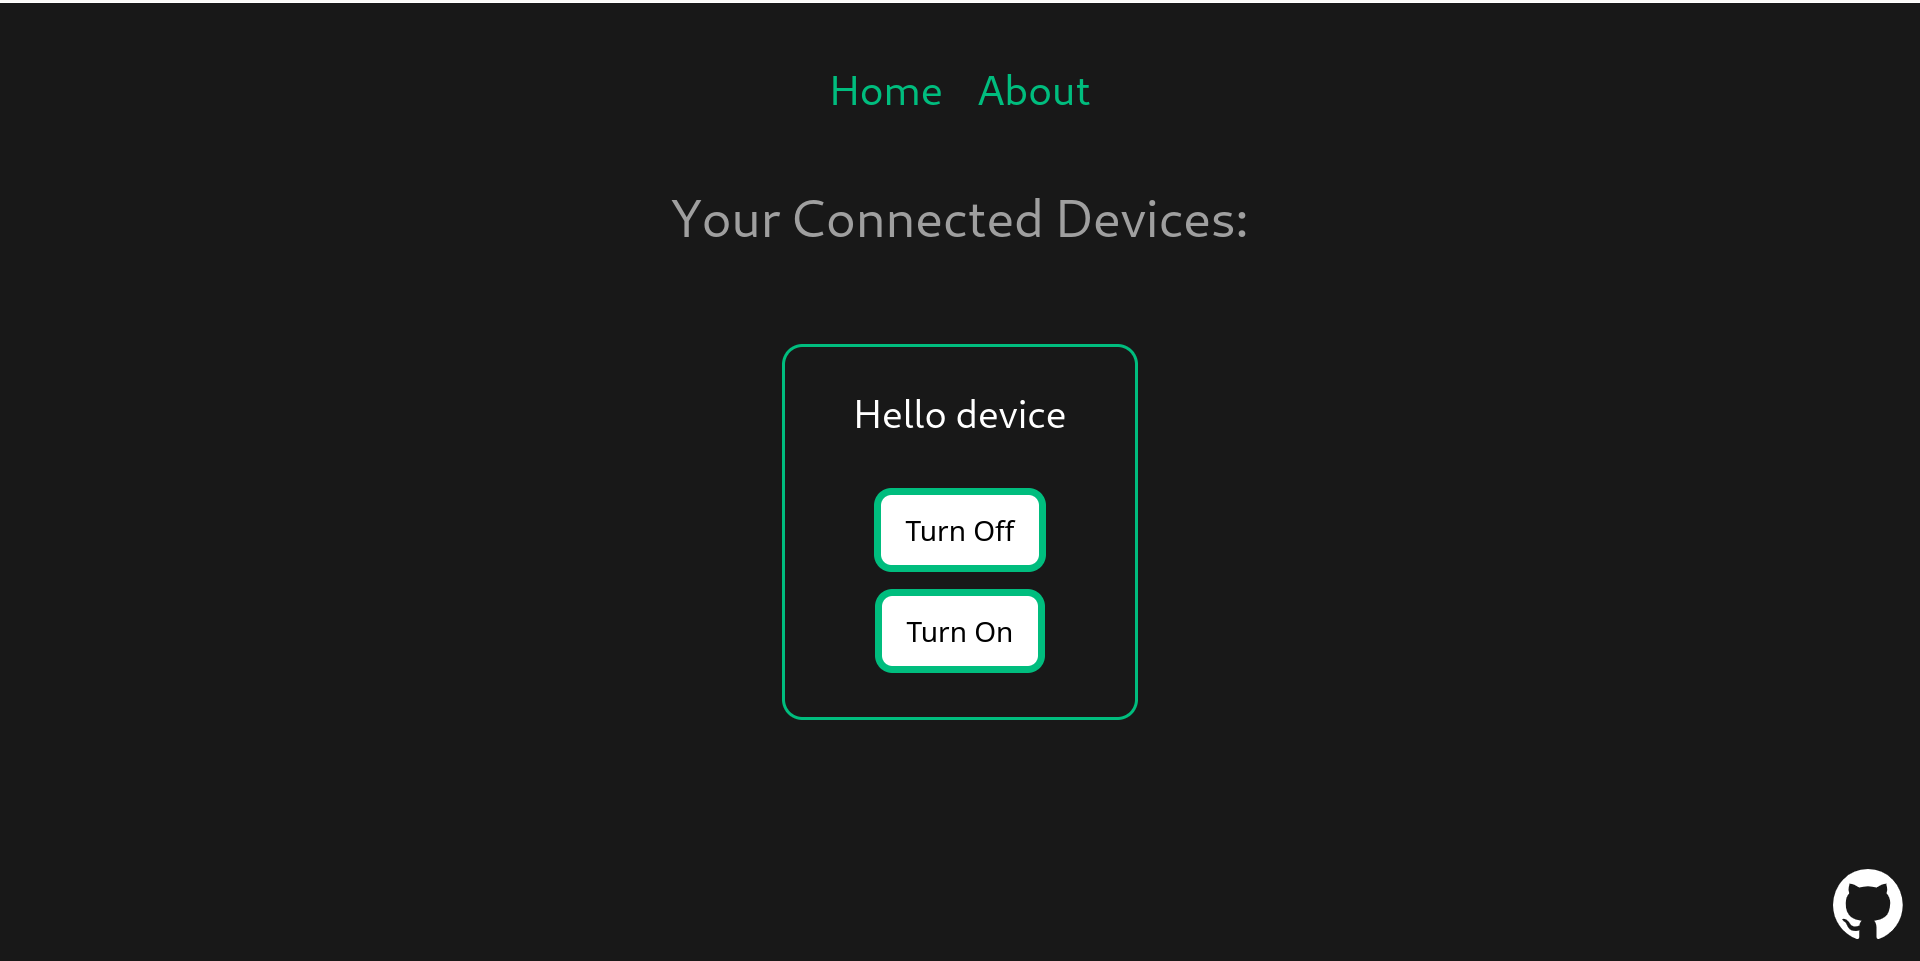
\includegraphics[width=\textwidth]{homescreen_final.png}
\label{fig:home_screen_final}
\end{figure}

The designs look fairly similar, with the only real difference being Github icon in the bottom right corner, that serves as a link to the project's repository. This allows the user easy access to documentation, or the ability to file a bug report in the Issues section of the repository.

\subsubsection{Calling the frontend API from the Web}
There are two ways to call the frontend API, one through JSON using an HTTP server, the second through gRPC. For the reasoning behind this view subsection~\ref{sec:chapimpl:frontend:json}. The web-frontend uses the JSON API to make calls to frontend API endpoints. All this means for a user of the system, is that they will need to start the server with the \textit{"-{}-json-frontend} flag, to enable the HTTP server that allows for JSON calls.

Once the HTTP server has been enabled, calling the frontend API is fairly easy. The vue\_frontend (which houses all web frontend files) contains a simple script which can used to generate JS files and with Typescript type definitions from the protobuf definitions.The script uses a Javascript library called ProtobufJs, to generate these files. Once these files are available, all types used in the CLI frontend are now also available, making calling the frontend API very easy. A typescript code snippet that shows how calls can be made to the JSON Proxy server can be seen in appendix section~\ref{chap:A2:apicallsjsonproxy}.


In this typescript snippet we construct a new "RegistrationRequest", which is defined the protobuf definition file from section~\ref{sec:chapimpl:server:protoBufs}, send it in the JSON format to the server. We then await a response and parse it into a "RegistrationResponse" and return that. The request is being made to the address "http://localhost:5173/api/frontend/registration" (defined in a constant, not visible in example). While at first this seems strange, as the JSON proxy is being hosted on address "http://localhost:2302", however due to the "/api" prefix in the address, the request is automatically forwarded to the HTTP server. This is handled by the Vite web server, which is hosting the website, which is being run when we call "npm run dev".

\subsection{Using JSON for the Frontend API} \label{sec:chapimpl:frontend:json}
Throughout this report a JSON frontend API has been alluded to, this subsection will explain why it was necessary to implement this in the first place. GRPC uses the HTTP/2 protocol to communicate, which is supported by web browsers. However, some features in HTTP/2 required by gRPC are not exposed by web browser \cite{grpcWeb} for a variety of reasons, which lead to the creation of gRPC web. GRPC web functions slightly differently to normal gRPC and is not compatible with normal gRPC, due to the aforementioned HTTP/2 issues. Because of this, a proxy between the normal gRPC server and gRPC web needs to be used to communicate.

Instead of using a separate program as a proxy, I decided to use a JSON to GRPC translation proxy instead, running on the server. This makes it possible to use a web-based frontend, without having the additional restrictions imposed by gRPC web. The downside of this, is that another HTTP server needs to be spawned, if the user decides to use JSON. Additionally, all benefits of using GRPC with the frontend are lost, as JSON is sent anyway. That being said, there are some benefits.

The JSON proxy I have created is completely transparent to the server, as the proxy calls gRPC functions. Additionally, the protobuf files are still used in combination with Typescript. This means that nothing in the packets is changed between the proxy and the server, the packet is simply parsed and forwarded as a gRPC packet. Another positive side effect of the JSON proxy, is that most frontend developers are significantly more familiar with working with JSON than gRPC, making it easier to create a custom frontend for the system. No extra program needs to be installed, or started when using a web-based frontend, one simply needs to include a flag when starting the server and the rest is handled automatically. Finally, if a user wants to create a web frontend using gRPC web, this can easily be done, with no changes required to the server code.

View an example below of how JSON calls to the server are translated to gRPC function calls (from the file \textit{\textbf{backend/src/server/web\_json\_translation/json\_registration.rs}}): 
\begin{lstlisting}[language=Rust, style=boxed, showstringspaces=false]{}
#[actix_web::post("/frontend/registration")]
pub async fn json_registration(
    req_body: String,
    state: actix_web::web::Data<TranslationClientState>,
) -> impl Responder {
    let parsed_req: 
        json_registration_service::RegistrationRequest =
            match serde_json::from_str(&req_body) {
                Ok(r) => r,
                Err(_e) => return 
                    HttpResponse::BadRequest()
                        .body("Unable to parse request"),
            };

    let response = {
        let mut registration_service_client 
            = state.registration_client.lock().await;

        registration_service_client
            .register(parsed_req).await
    };

    let response = match response {
        Ok(r) => r.into_inner(),
        Err(e) => return HttpResponse::InternalServerError()
            .body(e.to_string()),
    };

    return HttpResponse::Ok()
        .body(serde_json::to_string(&response).unwrap());
}
\end{lstlisting}
While this code looks complicated (partially due to formatting restrictions), it is actually quite simple. We parse the JSON request into a RegistrationRequest struct. If fails we send an error to the sender. We then forward the request to our "registration\_service\_client", which is a gRPC client registered as a frontend with the server. This is contained in a Mutex, due to the fact that it may be accessed concurrently, so we need to wait for it's lock to be available first. Finally, we check that the response is not an error. If it is not, we turn the response to a string and forward it to the sender, otherwise we forward the error message.

\section{Security} \label{sec:chapimpl:security}
This section will briefly showcase implementations of the protocols described within subsection~\ref{sec:chapdesign:security}. Both certificates and signatures are using an RSA key-pair generated by the Rust RSA library specifically the Probabilistic Signature Scheme (pss) module. From the private and public key we can generate a signing and verification key respectively. These are then used to sign and verify the certificates.

\subsection{Certificates} \label{sec:chapimpl:security:certificates}
Generating certificates is fairly simple, the code for this can be found in the file \textit{\textbf{backend/src/server/certificate\_signing.rs}}. We use the server's signing key to generate a digest of csr (described in section~\ref{sec:chapdesign:security}). We then store this certificate on the server side and send a copy to the device requesting to connect. To verify a certificate we simply use the verify function, present on the server's verification key.

\subsection{Signatures} \label{sec:chapimpl:security:signatures}
Signatures are similarly simple. To generate a signature for a message being sent we use the sign\_data function (from \textit{\textbf{backend/src/server/certificate\_signing.rs}}):
\begin{lstlisting}[language=Rust, style=boxed, showstringspaces=false]{}
///returns the signature and timestamp of the signature
pub fn sign_data(&self, data: String) -> (Vec<u8>, u64) {
    let timestamp = get_timestamp();
    let data = timestamp.to_string() + &data;

    let mut rng = rand::thread_rng();
    let signed = self.signing_key.sign_with_rng(
        &mut rng, data.as_bytes()
    );
    (signed.to_vec(), timestamp)
}
\end{lstlisting}
As mentioned in the comment on line one, this function takes data in the form of a string, concatenates it with the current time-stamp (in Unix time), then signs it with the same pss signing key used to generate certificates. It then returns the signature in the form of an Array of bytes, along with the timestamp.

Due to more complexity in the verification function, it will be provided in pseudo code. For the original Rust code, view the file \textit{\textbf{backend/src/server/certificate\_signing.rs}}. 
\begin{lstlisting}[language=Python, style=boxed, showstringspaces=false]{}
def verify_signature_update_request(
    client_verifying_key,
    certificate,
    updated_capabilities,
    client_timestamp
    signature
):
    server_timestamp = get_timestamp()
    if (
        server_timestamp - client_timestamp 
        > SIGNATURE_EXPIRATION_SECONDS
    ):
        return false

    capability_string = updated_capabilities.reduce(
        (acc, capability) => {
            acc + capability.to_string()
        }
    )
    to_check_against = client_timestamp 
        + capability_string
        + certificate

    return client_verifying_key.verify(
        to_check_against,
        signature
    )
\end{lstlisting}
The signature verification function uses the client's verification key, derived from the client's public key, to verify that the signature is genuine. Included in the signatureis the time the message was sent (view sections~\ref{sec:chapdesign:security}) The current expiration time for a signature (and in extension a message) is 10 seconds. This ensures that an attacker cannot use a replay attack to maliciously control the system and if something goes wrong during packet transfer, that outdated packets don't influence behavior. 



\newpage
\chapter{Testing \& Evaluation} \label{cha:testing}
\section{Using the System}
To test Aims and Objectives 1 \& 2, \todo{finish this section}

for All tests in this section a Raspberry Pi 4b was used to host client code, running Raspberry Pi OS Lite (with no desktop environment), which was released on December 11th 2023. The server and frontend were hosted on a Laptop with an Intel i5-12450H processor, running Fedora 39 Linux. The Raspberry Pi's hostname (visible in screenshots) is "nikpi".
\subsection{Controlling one connected device} \label{cha:testing:onedevice}
Perhaps the most obvious and basic test is to create a device, using the Rust client library, have it run on a device and to connect with that device to a running server. 

\subsubsection{Testing Setup}
A simple client was created, with two capabilities "Turn On" and "Turn Off". The callback functions attached to these capabilities would simply log to the standard output the name of the capability they are attached to. The Raspberry Pi is connected to the same Wi-Fi network as the server. The port 2302 has opened on the laptop's firewall to ensure the Raspberry Pi can make requests to the gRPC server. The Raspberry Pi is being controlled through a secure shell connection (SSH) (visible on the left side of screenshots). View figure~\ref{fig:example_config_raspi} for the exact configuration of the client.
\begin{figure}[h]
\caption{Client's configuration file}
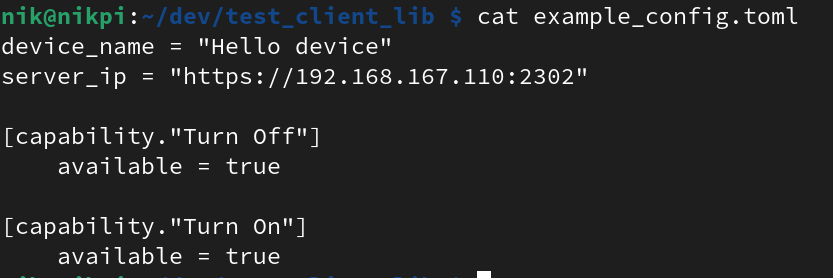
\includegraphics[width=\textwidth]{example_config_raspi}
\label{fig:example_config_raspi}
\end{figure}

\subsubsection{Testing}
Figure~\ref{fig:establish_connection_raspi} shows the successful connection and certificate exchange between the client on nikpi and the server. Note that the server ip that the client is connecting to is set within the client's configuration file (view figure~\ref{fig:example_config_raspi}). In this case the server (on the right side of figure~\ref{fig:establish_connection_raspi}) is being started with the "json-frontend" flag, as discussed within subsection~\ref{sec:chapimpl:frontend:json}, this flag is required to use the web-based frontend.
\begin{figure}[h]
\caption{Establishing a connection }
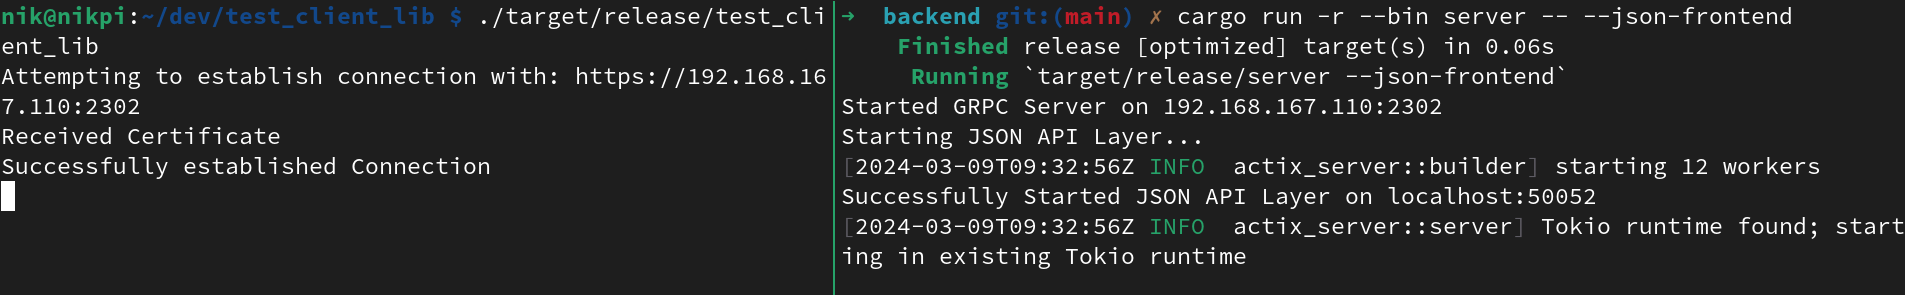
\includegraphics[width=\textwidth]{establish_connection_raspi}
\label{fig:establish_connection_raspi}
\end{figure}

The next important test is viewing the web frontend, to see that the device is correctly displayed on the frontend, with the appropriate capabilities. This can be seen in figure~\ref{fig:web_frontend_one_connected_device}, where the device, named "Hello device" (view configuration file) can be seen with it's two capabilities "Turn Off" and "Turn On". The web-frontend is being hosted by a Vite server, through using the command "npm run dev", on localhost port 5173. The frontend is being rendered by the Chromium web browser.
\begin{figure}[h]
\caption{Web Frontend with the connected device}
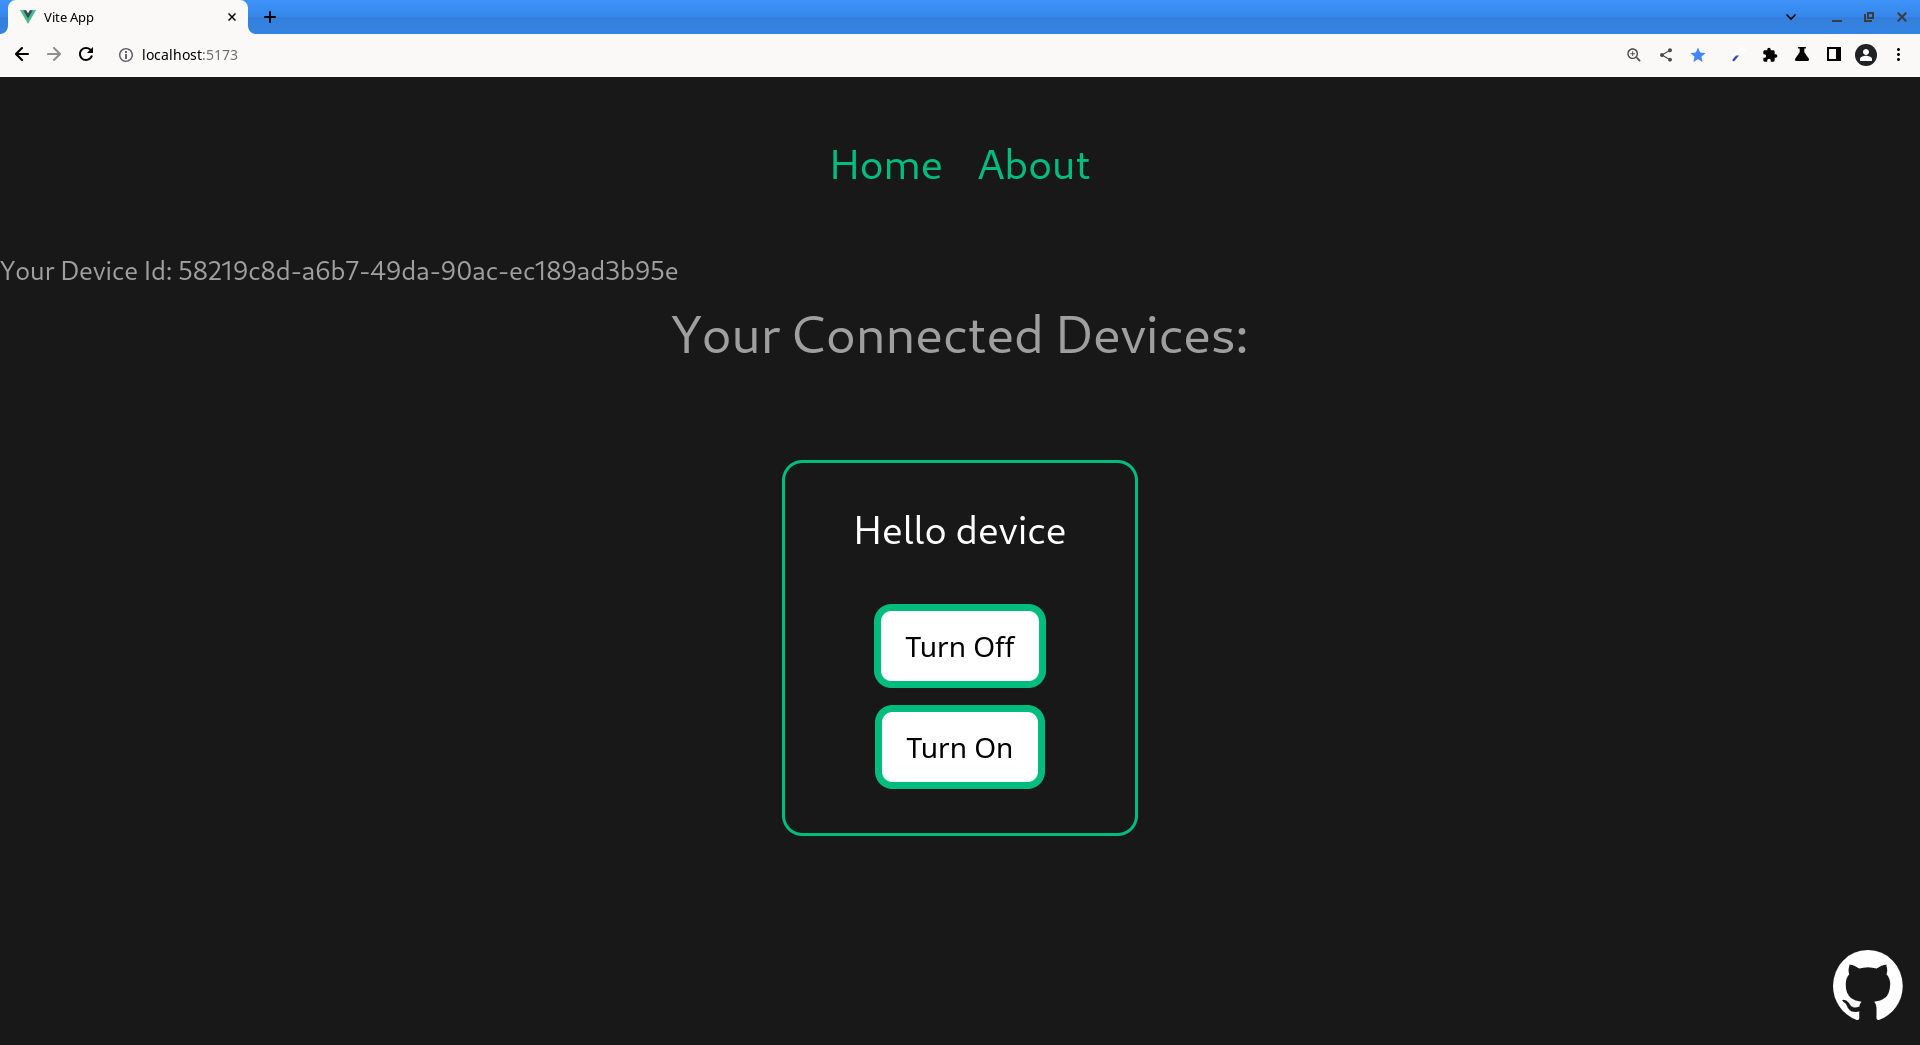
\includegraphics[width=\textwidth]{testing_web_frontend_one_device}
\label{fig:web_frontend_one_connected_device}
\end{figure}

The final test for this subsection is to attempt to trigger the two listed capabilities, by clicking the buttons. This should send a JSON packet to the JSON proxy server, which is then forwarded to the gRPC server. Once this request has been processed, the server will add it to the list of updates for the specified client. The client will then eventually poll the server and receive the update. It will then call the callback function associated with that capability. For this specific test both buttons will be clicked, starting with the "Turn Off" button, then the "Turn On Button". As shown in figure~\ref{fig:triggering_capability} this works as expected and the associated callback functions are called.
\begin{figure}[h]
\caption{Triggering capabilities}
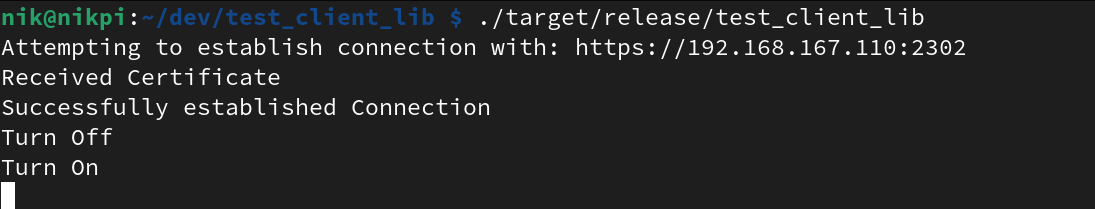
\includegraphics[width=\textwidth]{toggle_turn_on_off}
\label{fig:triggering_capability}
\end{figure}

You can view the complete code for the client used in this example in the appendix. Due to the simplicity of setting up a client using the NOSHP-Client library, its only 47 lines long.

\subsection{Running with One connected Device over Wifi} 
\subsection{Running with multiple connected devices}
\subsection{Sending incorrect signatures}
\section{Performance Testing}


\newpage
\chapter{Conclusion} \label{cha:conclusion}


%%
%% You bib file
%%
\newpage
\bibliography{report}

\newpage
\appendix
%%
%% Your appendices
%%
\chapter{Original Project Proposal}
\label{chap:A1}

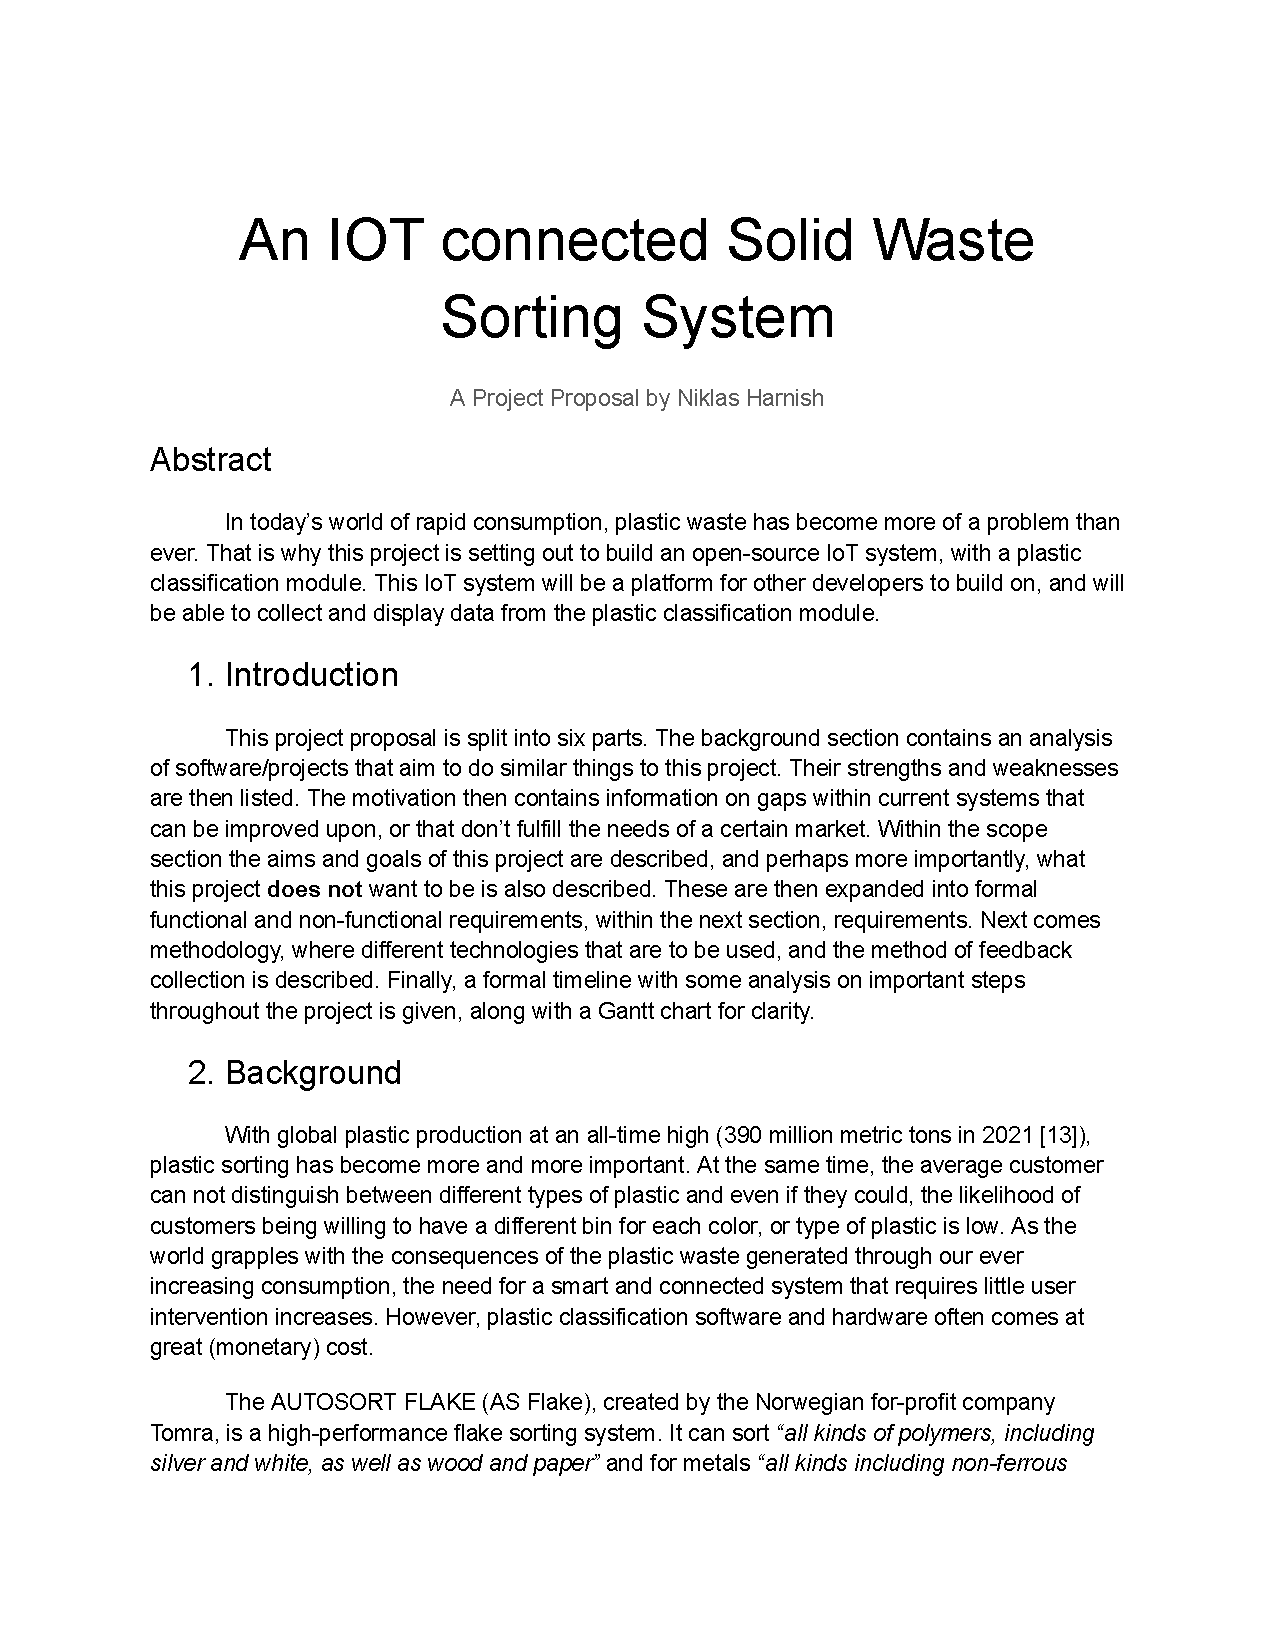
\includepdf[pages=-]{project_proposal.pdf}

\newpage

\chapter{Another Appendix Chapter}
\label{chap:A2}

This could be about your experiments

\end{document}
